\documentclass[final]{fhnwreport}       %[mode] = draft or final
                                        %{class} = fhnwreport, article, 
                                        %          report, book, beamer, standalone
%%---Main Packages-----------------------------------------------------------------------
\usepackage[english, ngerman]{babel}	%Mul­tilin­gual sup­port for LaTeX
\usepackage[T1]{fontenc}				%Stan­dard pack­age for se­lect­ing font en­cod­ings
\usepackage[utf8]{inputenc}				%Ac­cept dif­fer­ent in­put en­cod­ings
\usepackage{lmodern}                    %The newer Font-Set
\usepackage{textcomp}					%LaTeX sup­port for the Text Com­pan­ion fonts
\usepackage{caption}					%Customising captions in floating environments

\usepackage{graphicx} 					%En­hanced sup­port for graph­ics
\usepackage{float}						%Im­proved in­ter­face for float­ing ob­jects
\usepackage{ifdraft}                    %Let you check if the doc is in draft mode

%%---Useful Packages---------------------------------------------------------------------
\usepackage{color}						%Colour control for LaTeX documents
\usepackage[pdftex,dvipsnames]{xcolor}  %Driver-in­de­pen­dent color ex­ten­sions for LaTeX
\usepackage{csquotes}                   %Simpler quoting with \enquote{}
\usepackage{siunitx} 					%A com­pre­hen­sive (SI) units pack­age
\usepackage{listings}					%Type­set source code list­ings us­ing LaTeX
\usepackage[bottom]{footmisc}			%A range of foot­note op­tions
\usepackage{footnote}					%Im­prove on LaTeX's foot­note han­dling
\usepackage{verbatim}					%Reim­ple­men­ta­tion of and ex­ten­sions to LaTeX ver­ba­tim
\usepackage[textsize=footnotesize]{todonotes} %Mark­ing things to do in a LaTeX doc­u­ment
\usepackage{titling}					%Control over the typesetting of the \maketitle command

\usepackage{float}
\usepackage{wrapfig}

%%---Tikz Packages-----------------------------------------------------------------------
\usepackage{standalone}
\usepackage{tikz}
\usepackage{circuitikz}
\usetikzlibrary{arrows}
\usetikzlibrary{calc}
\usetikzlibrary{intersections}

%%---Math Packages-----------------------------------------------------------------------
\usepackage{amsmath}					%AMS math­e­mat­i­cal fa­cil­i­ties for LaTeX
\usepackage{amssymb}					%Type­set­ting symbols (AMS style)
%\usepackage{amstext}
%\usepackage{amsfonts}
%\usepackage{breqn}
\usepackage{array}						%Ex­tend­ing the ar­ray and tab­u­lar en­vi­ron­ments
\usepackage{amsthm}					%Type­set­ting the­o­rems (AMS style)

%%---Table Packages----------------------------------------------------------------------
\usepackage{tabularx}					%Tab­u­lars with ad­justable-width columns
%\usepackage{longtable}
\usepackage{multirow}					%Create tab­u­lar cells span­ning mul­ti­ple rows
\usepackage{multicol}					%In­ter­mix sin­gle and mul­ti­ple columns

%%---PDF / Figure Packages---------------------------------------------------------------
\usepackage{pdfpages}					%In­clude PDF doc­u­ments in LaTeX
\usepackage{pdflscape}					%Make land­scape pages dis­play as land­scape
\usepackage{subfig}					    %Fig­ures di­vided into sub­fig­ures

%%---Other Packages----------------------------------------------------------------------
%\usepackage{xargs}                     %De­fine com­mands with many op­tional ar­gu­ments


%%---Bibliography------------------------------------------------------------------------
\usepackage[style=ieee,urldate=comp,backend=biber]{biblatex}
\addbibresource{literature/bibliography.bib}

%%---Main Settings-----------------------------------------------------------------------
\graphicspath{{./graphics/}}			%Defines the graphicspath
\geometry{twoside=false}				    %twoside=false disables the "bookstyle"
\setlength{\marginparwidth}{2cm}
\overfullrule=5em						%Creates a black rule if text goes over the margins => debugging




%%---User Definitions--------------------------------------------------------------------
%%Tabel-Definitions: (requires \usepackage{tabularx})
\newcolumntype{L}[1]{>{\raggedright\arraybackslash}p{#1}}    %column-width and alignment
\newcolumntype{C}[1]{>{\centering\arraybackslash}p{#1}}
\newcolumntype{R}[1]{>{\raggedleft\arraybackslash}p{#1}}

%%---Optional Package Settings-----------------------------------------------------------
%Listings-Settings: (requires \usepackage{listings}) => Example with Matlab Code
\lstset{language=Matlab,%
    basicstyle=\footnotesize\ttfamily,
    breaklines=false,%
    morekeywords={switch, case, otherwise},
    keywordstyle=\color{Blue},%
    tabsize=2,
    %morekeywords=[2]{1}, keywordstyle=[2]{\color{black}},
    identifierstyle=\color{Black},%
    stringstyle=\color{Purple},
    commentstyle=\color{Green},%
    showstringspaces=false,%without this there will be a symbol in the places where there is a space
    numbers=left,%
    numberstyle={\tiny \color{black}},% size of the numbers
    numbersep=9pt, % this defines how far the numbers are from the text
    %emph=[1]{word1, word2,...},emphstyle=[1]\color{red}
}							

%Hurenkinder und Schusterjungen verhindern (kein Scherz, Google es)
\clubpenalty10000
\widowpenalty10000
\displaywidowpenalty=10000	



%Titel mit Mathematik immer fett drucken
\usepackage{sectsty}
\allsectionsfont{\boldmath}




			                %loads all packages, definitions and settings											
\title{Fachbericht}  		        %Project Title
\author{Team 1}      				    %Document Type => Technical Report, ...
\date{\today}          				   %Place and Date

\begin{document}

%%---TITLEPAGE---------------------------------------------------------------------------------
\thispagestyle{empty}
%	\ohead{\includegraphics[scale=0.5]{Bilder/Logo_FHNW.jpg}}
	\begin{figure}
		 \vspace*{-\topskip}\vspace*{-\headsep}
		
\includegraphics[scale=1]{graphics/fhnw_ht_logo_de.pdf}
	\end{figure}
	\begin{center}
		\vspace*{2cm}
		{\huge{\textbf{digitales Theremin}}}\\
		\vspace*{0.2cm}
		{\huge{\textbf{\thetitle}}}\\
		\vspace*{0.5cm}
		
		{\scshape\Large Projekt 6\\} \Large{\today}
		\vfill
		\begin{normalsize}
			{\begin{tabbing}
					\textbf{Auftraggeber:} \hspace{5cm}\= Prof. Dr. Hanspeter Schmid\\
					
					\\[0.8cm]
					\textbf{Betreuung:} 
					\>Prof. Dr. Hanspeter Schmid\\
					\>Herr Prof. Karl Schenk\\


					\\[0.8cm]
					\textbf{Team:} \>Andreas Frei \\ \>Dennis Aeschbacher \\ 

					\\[0.8cm]
					\textbf{Studiengang:} \>Elektro- und Informationstechnik
					\\[0.8cm]	\textbf{Semester:} \>Frühlingssemester 2020
			\end{tabbing}}
		\end{normalsize}
		\vfill
	\end{center}
\clearpage
			
%%---ABSTRACT----------------------------------------------------------------------------
\selectlanguage{english}				%ngerman or english
\thispagestyle{empty}
\begin{abstract}
% Description aim/objective
\noindent In this Project a Theremin was built that mainly operates on digital hardware unlike the original device that solely used analog electronics. The device is supposed to be used in presentations for trade fairs by the Institute for Sensors and Electronics ISE. As such the device should be built in a appealing housing. Moreover the device should have other additional functionality such as soundeffects or the ability to record sound.
% Method
The digital hardware was implemented in VHDL on the developer board DE1-SoC from terasIC with a Cyclone V FPGA from Intel. The sole analog component implemented was the oscillator that controls the pitch. 
% Results
The pitch of the device can be changed well, but the sound itself has a flaw at the moment, because there is an audible crackle. This is due to a communication problem with the codec that was used for the audio output. This problem will not be corrected during this project, because the communication will be implemented differently in the finished product.
% Conclusion
The work in this project served as a platform for the continuation in project 6. The next steps would be to implement the volume control and redesign the pcb for two antennas and oscillators.


\end{abstract}	



%%---TABLE OF CONTENTS-------------------------------------------------------------------
\pagenumbering{Roman}		
\selectlanguage{ngerman}				%ngerman or english
\tableofcontents
\clearpage

%%---TEXT--------------------------------------------------------------------------------
\pagenumbering{arabic}
\clearpage
\section{Einleitung}\label{sec:Einleitung}
Das Theremin kennen heutzutage nur wenige Leute, obwohl es das erste elektronische Instrument war. Es wurde 1920 von dem Russen Lev Sergejewitsch Termen, welcher sich später zu Leon Theremin umbenennen liess, erfunden \cite{Theremin_h}. Personen die regelmässig Filme schauen, haben die Musik welche mit einem Theremin gemacht wird bestimmt schon einmal gehört. Ein Beispiel dafür ist Ghostbusters, wo das Theremin oft im Hintergrund zu hören ist. Zudem ist das Theremin in einigen Science-Fiction-Filmen und Horrorfilmen zu hören \cite{Goast_m}. Das Theremin wird ohne es zu berühren gespielt, indem man mit den Händen die Distanz zu zwei Antennen ändert. Dies führt zu Veränderung der Tonhöhe und Lautstärke.

Im Projekt 5 und 6 soll nun ein solches Instrument entwickelt werden. Mit dem Unterschied, dass das sonst analoge Instrument digital aufgebaut werden soll. Dabei soll es auf einem Field Programmable Gate Array (FPGA) implementiert werden. Später soll das Theremin als Messeobjekt für das Institut für Sensorik und Elektronik ISE verwendet werden. Im Rahmen des Projekt 5 wurde die Tonhöhenantenne des Theremin realisiert. Dazu wurde die Antenne zusammen mit dem Antennenoszillator analog beibehalten. Die restlichen Komponenten wurden in VHDL realisiert. Das Resultat wurde auf dem DE1-SoC Board von terasIC mit einem Cyclone V FPGA von Intel getestet.

Der folgende Fachbericht beginnt mit dem Kapitel \ref{sec:Technische Grundlagen} Technische Grundlagen.In der ersten Hälfte des Kapitel wird erklärt wie ein analoges Theremin funktioniert und welche Komponenten ein Theremin ausmachen. In der zweiten Hälfte werden digitale Lösungsansätze besprochen. Anschliessend wird im Kapitel \ref{sec:Realisierung} Realisierung beschrieben wie die Komponenten realisiert wurden. Im Kapitel \ref{sec:Validierung} Validierung wird als erstes auf die Inbetriebnahme des Antennenoszillators eingegangen. Als nächstes werden die Simulationen des VHDL Codes erläutert. Im letzten Abschnitt wird auf die Inbetriebnahme des VHDL Codes auf dem DE1-SoC Board Bezug genommen.






\pagebreak

	
\clearpage
\section{Technische Grundlagen}\label{sec:Technische Grundlagen}
Um ein Verständnis für dessen Funktionsweise zu gewinnen, ist in diesem Kapitel als erstes erklärt, wie ein analoges Theremin funktioniert. Anschliessend folgt ein kleiner Abschnitt zur Musiktheorie. Zuletzt werden verschiedene Algorithmen erklärt, welche im digitalen Theremin eingesetzt wurden.
	\subsection{analoges Theremin}\label{subsec:Theremin_analog}
Das klassische Theremin besitzt zwei Antennen. Der Spieler kann über die senkrecht angebrachte Antenne  die  Tonhöhe beeinflussen. Mit der waagrechten Antenne beeinflusst der Spieler die Lautstärke. Eine typische Eigenschaft des Theremin ist, dass der Ton des Theremin in einem weitem Frequenzbereich kontinuierlich veränderbar ist. Das Theremin kann daher alle Frequenzen in einem Bereich spielen, im Gegensatz zu den meisten anderen Instrumenten.

Der Spieler spielt das Theremin durch verstimmen der Oszillatoren über die Antennen.
Die Hand des Spielers verändert über die jeweilige Antenne die Schwingfrequenz des Tonhöhen und Lautstärkeoszillators. Dabei wird der kapazitive Anteil des LC-Schwingkreises beeinflusst, was eine Änderung der Schwingfrequenz zur Folge hat. 
Die Frequenz dieser Oszillatoren ist jedoch weit über dem hörbaren Bereich (zwischen \SI{100}{kHz} bis \SI{1}{MHz}). Mit Hilfe eines Mischers und einem Referenzoszillator wird die Frequenzdifferenz des Tonhöhenoszillators hörbar gemacht und danach verstärkt\cite{Franzis}. Der Lautstärkepegel ergibt sich durch die Verwendung eines Bandpassfilters und nachfolgenden Hüllkurvendetektor. Die Abbildung \ref{img:Blockschaltbild_analog} gibt einen Überblick über die Schaltungskomponenten eines Theremins. Die einzelnen Schaltungsteile sind im folgenden Teil genauer erklärt.

\begin{figure}[h]
	\centering
	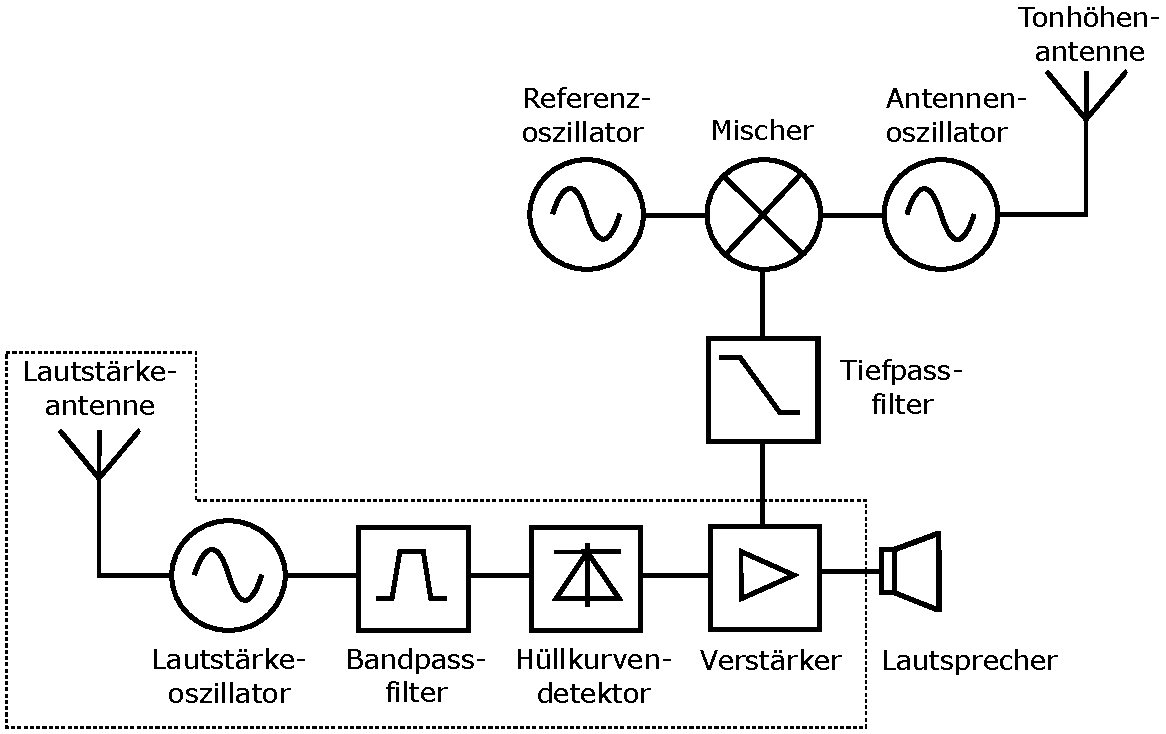
\includegraphics[width=0.8\textwidth]{Blockschaltbild_analog.pdf}
	\caption{Blockschaltbild eines analogen Theremins}
	\label{img:Blockschaltbild_analog}
\end{figure}

\paragraph{Tonhöhenoszillator und Tonhöhenantenne}\mbox{}\\

Die Tonhöhenantenne ist ein Metallrohr welches mit dem Tonhöhenoszillator verbunden ist.
Der Spieler kann über die Distanz seiner Hand zur Antenne die Frequenz des Tonhöhenoszillator verändern. Die über die Antenne zu erreichende Kapazitätsänderung ist sehr gering. Diese liegt im Picofarad Bereich \cite{physik_theremin}.Die Grundfrequenz des Tonhöhenoszillator muss weit über dem hörbaren Bereich liegen, dass eine genügend grosse Frequenzänderung entsteht.

\paragraph{Lautstärkeoszillator und Lautstärkeantenne}\mbox{}\\ 

Die Lautstärkeantenne ist wie die Tonhöhenantenne ein Metallrohr, welches mit dem Lautstärkeoszillator verbunden ist. Die durch den Spieler beeinflusste Frequenzänderung wandelt ein Hüllkurvendetektor in eine Spannung um. Diese Spannung dient dem Verstärker als Steuergrösse um das Audio Signal zu verstärken. \cite{Franzis}. 

\paragraph{Mischer und Referenzoszillator}\mbox{}\\ 
\\Die erzeugte Frequenz der Tonhöhenantenne ist weit über dem vom Menschen hörbaren Bereich. Der Mischer multiplizeirt die Signale des Referenzoszillators und des Tonhöhenoszillators wie in Formel \ref{equ:mischer}. $A_1\sin(\omega_1)$ ist das Signal des Referenzoszillators und $A_2\sin(\omega_2)$ das Signal des Tonhöhenoszillators.

\begin{equation}
V_{out} = A_{1}A_{2} \sin(\omega_{1}t)   \sin(\omega_{2}t) 
\label{equ:mischer}
\end{equation}

$V_{out}$ kann durch Additionstheoreme umgeformt werden. Dabei erhält man folgenden Ausdruck:

\begin{equation}
V_{out} = A/2[\cos((\omega_{1}-\omega_{2})t)  - \cos((\omega_{1}+\omega_{2})t) ]
\label{equ:mischer_trigo}
\end{equation}

Das Ausgangssignal $V_{out}$ hat zwei Frequenzkomponenten. Zum einen die Differenz der beiden Frequenzen zum anderen die Summe der Frequenzen. Dabei ist bei dem Theremin nur die Differenz der Frequenzen von Interesse \cite{physik_theremin}.

Eine Kalibration des Theremins ist vor jedem Gebrauch nötig. Es könnte beispielsweise sein, dass die Differenz der Frequenz ausserhalb des hörbaren Bereiches ist. Dazu stellt der Spieler beim klassischen Theremin mit Hilfe eines Trimmkondensators am Referenzoszillator die Differenzfrequenz auf \SI{0}{Hz} ein.

\paragraph{Tiefpassfilter}\mbox{}\\ 
\\Das Tiefpassfilter filtert die hochfrequente Komponente aus Formel \ref{equ:mischer_trigo} weg. Übrig bleibt die Differenz der Oszillatorfrequenzen. Dieser ist der interessante Anteil des Mischprozesses, da er im hörbaren Bereich ist.
\begin{equation}
V_{out} = A/2cos((\omega_{1}-\omega_{2})t) 
\label{equ:mischer_gefilt}
\end{equation}

\paragraph{Verstärker und  Lautsprecher}\mbox{}\\ 
\\Der Verstärker verstärkt das Ausgangssignal des Tiefpassfilter abhängig von der Spannung, welche vom Hüllkurvendetektor stammt.

	\subsection{digitales Theremin}\label{subsec:Theremin_digital}

bla bla







\clearpage
\section{Realisierung}\label{sec:Realisierung}

Das digitale Theremin ist auf dem Entwicklungsboard DE1-SoC von Terasic aufgebaut. Dieses enthält ein Cyclone V 5CSEMA5 FPGA von Intel. Weiter befindet sich auf dem Board der Audio Codec WM8731 von Wolfson für die Ausgabe an einem Lautsprecher. In Abbildung \ref{img:Blockschaltbild_top} ist der Aufbau des digitalen Theremin aufgezeigt inklusive der Peripherie ausserhalb des FPGA.\\
Das Theremin, welches im FPGA aufgebaut ist, besteht aus zwei Bereichen. Einerseits der Signalverarbeitung und Übermittlung an den Codec. Dieser besteht aus den Komponenten \textit{Lautstärken}- und \textit{Tonhöhenverarbeitung}, \textit{DC-FIFO} und dem \textit{Audioserialisierer}. Der zweite Bereich ist das Nios II System. Dieses besteht aus dem Prozessor und diversen IP Cores, welche die Kommunikation mit den Peripherien ermöglicht. Ausserhalb des FPGA befindet sich zudem das entwickelte PCB, welches die beiden Antennenoszillatoren enthält und das Spielen des Theremins ermöglicht.\\
Die Kommunikation zwischen dem Nios II Prozessor und den anderen Komponenten geschieht über das \textit{Avalon Memory Mapped Interface}. Der Prozessor agiert in dieser Kommunikation als Master und die restlichen Komponenten als Slaves. Die Übertragung der Audioinformation in der Signalverarbeitung geschieht über das \textit{Avalon Streaming Interface}. Wobei Sender als Streaming Source und Empfänger als Streaming Sink deklariert sind. Das Streaming Interface ist notwendig für den Einsatz des Dual-Clock-FIFO (DC-FIFO). Dieses übernimmt den Übergang verschiedener Clockregionen zwischen den Komponenten \textit{Tonhöhenverarbeitung} und \textit{Audioserialisierer}.\\
Die Clocks, welche zu den verschiedenen Komponenten führen sind in Abbildung \ref{img:Blockschaltbild_top} für eine bessere Übersichtlichkeit weggelassen worden. Für eine Liste aller Clock Frequenzen und deren Ziel siehe Kapitel \ref{subsec:Clock}.

\begin{figure}[h!]
	\centering
	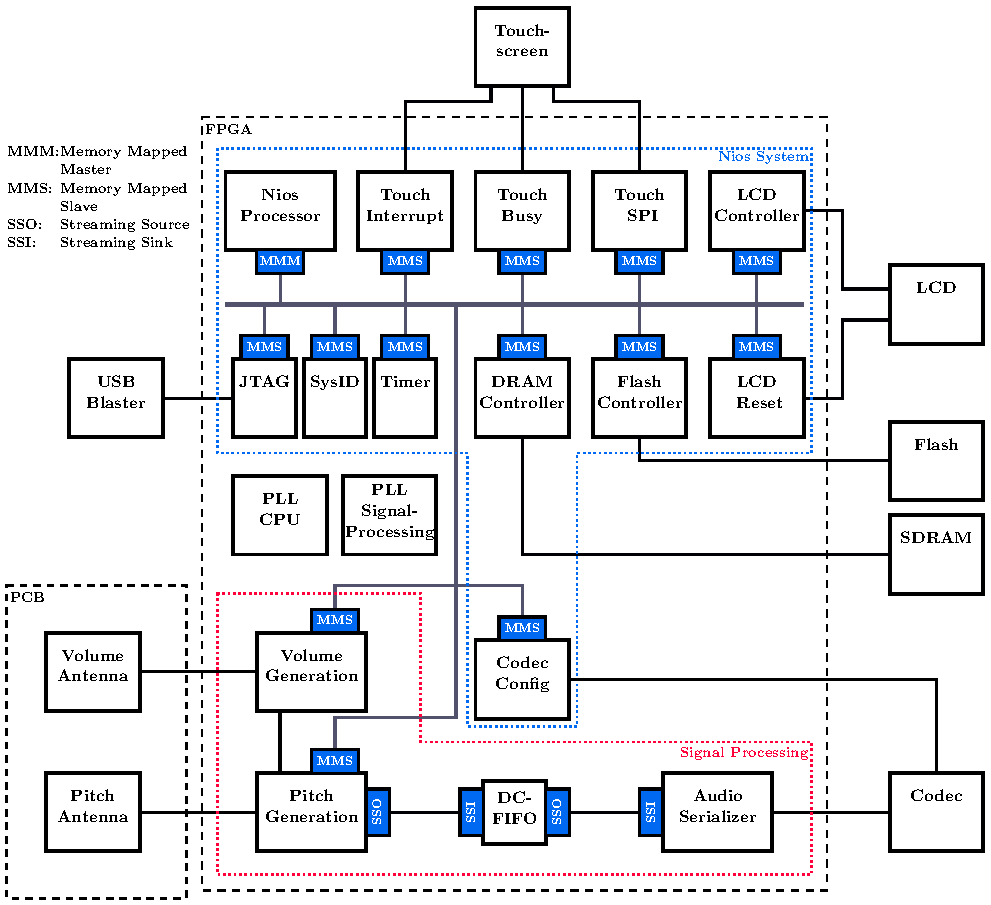
\includegraphics[width=1\textwidth]{Blockschaltbild_top.pdf}
	\caption{Blockschaltbild gesammtes Theremin} 
	\label{img:Blockschaltbild_top}
\end{figure}  

\clearpage


	\subsection{Tonhöhen- und Lautstärkenoszillator}\label{subsec:Antennenoszilator}
Für die Antennenoszillator-Schaltung haben wir uns im Projekt 5 für den Colpitts-Oszillator aus Abbildung \ref{img:colpitts} entschieden. Der Aufbau im Projekt 5 umfasste nur einen Oszillator zur Veränderung der Tonhöhe.

Es handelt sich dabei um einen Colpitts-Oszillator mit einem JFET. Diese Schaltung ist von dem Bauset ''Theremin selber bauen`` von Franzis übernommen \cite{Franzis}. 
Da der im Bauset verwendete JFET nicht mehr bestellbar ist, war ein Wechsel auf den J113 N-Kanal JFET nötig. Die mit LTspice simulierten Werte des J113 glichen stark der Originalschaltung, weshalb der Entscheid auf diesen fiel. 
Damit das Sinussignal des Antennenoszillator nicht A/D gewandelt werden muss, wandelt eine Komparatorschaltung das Sinussignal in ein Rechtecksignal mit gleicher Frequnez um. 
Diese ist mit \SI{3.3}{V} betrieben, da die Logikeingänge des FPGA auf diese Spannung ausgelegt sind. 

Im Projekt 5 wurde als Antenne ein Messingrohr verwendet. Diese ist am Anschluss pitch\_antenna verbunden. 

Die Ausgangsspannung des Colpitts-Oszillator ist über den Kondensator C11 entkoppelt. Dies entfernt den DC-Anteil. Der Kondensator C11 und die Widerstände R3 und R4 bilden zusammen einen Hochpass. Damit die Oszillatorfrequenz von ca \SI{562}{kHz} das Filter passieren kann, ist C11 so gewählt, dass die Grenzfrequenz des Filters bei ca \SI{265}{kHz} liegt. 

Auf dem PCB sind nun im Projekt 6 zwei solche Oszillatoren verbaut: Der Tonhöhenoszillator und der Lautstärkenoszillator. Das PCB ist mit einem \SI{12} {VDC} Schaltnetzteil gespiessen. Der MC7809 Spannungsregler generiert die \SI{9} {VDC} für die Colpitts-Oszillatorschaltungen. Die \SI{3.3} {VDC} für den Komperator erzeugt der LT1117 Spannungsregler. Bei der Wahl der Spannungsregler ist darauf geachtet worden, dass die erzeugten Spannungen möglichst störungsfrei ist und wenig Ripple aufwiesen. Das gesamte Schema der Schaltung ist im Anhang enthalten.

\begin{figure}[h]
	\centering
	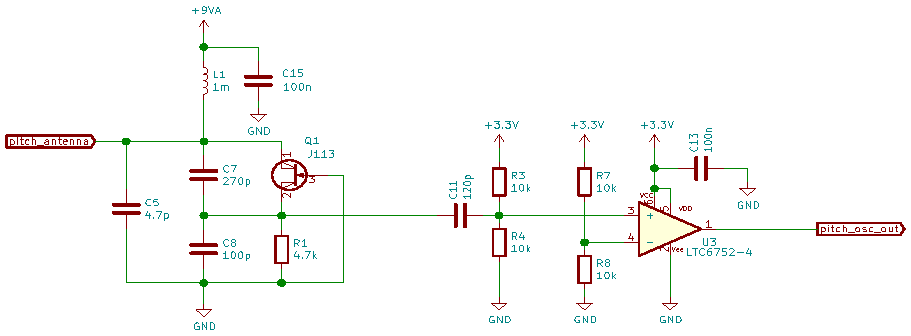
\includegraphics[width=\textwidth]{colpitts.pdf}
	\caption{Schema Antennenoszillator. Links Collpitts-Oszillator, rechts Komparatorschaltung}
	\label{img:colpitts}
\end{figure} 

\clearpage



	\subsection{Clock}\label{subsec:Clock}
Die verschiednen Clocks für die Hardwarekomponenten und die CPU werden in zwei PLL Blöcken generiert. Ein Block für die Signalverarbeitung und einer für das Nios System. In Tabelle ... \todo{Referenz einfügen} sind alle Frequenzen aufgelistet. 

\todo{Tabelle mit allen Frequenzen einfügen}


	\subsection{Nios II System}\label{subsec:CPU}
Der eingesetzte Nios II Prozessor ist für die Bedienung des Theremin und die Steuerung der Signalverarbeitungshardware zuständig. Die diversen eingesetzten IP Cores sind in den unten stehenden Kapiteln beschrieben.

\paragraph{JTAG, Timer und System ID}\mbox{}\\

Der JTAG IP Core ermöglicht das flüchtige Programmieren des Nios II wie auch das Kommunizieren mit selbem für Debugging Zwecke. 
Durch den Einsatz des Timer IP Cores erhält der Nios II einen Interval Timer, um beispielsweise periodisch Interrupts zu generieren. 
Im System ID IP Core ist die Systemidentifikationsnummer gespeichert. Diese ist nötig, um beim Laden der Software sicherzustellen, dass das passende Hardware Image vorhanden ist.
Alle drei Komponenten sind mit Standardeinstellungen in das Nios II System eingefügt worden.

\paragraph{Speicher}\mbox{}\\

Der Arbeitsspeicher ist ein externer 64MB SDRAM Chip IS42S16320D von ISSI. Für die Kommunikation mit dem Nios II Prozessor ist der SDRAM Controller IP Core zuständig. Der Nios II Prozessor kann über das Memory Mapped Interface mit dem Core kommunizieren und so auf das SDRAM zugreifen. Da dieser Chip bereits auf dem Entwicklungsboard vorhanden ist und um Ressourcen zu sparen, haben wir uns gegen On-Chip Speicher entschieden.\\

Das Hardware Image und der Programmcode sind auf dem Board enthaltenen Flash Speicher gespeichert. Dabei lädt Quartus, anders als bei dem nicht flüchtigen Programmieren, nicht das SRAM Object File (.sof) sondern ein JTAG Indirect Configuration File (.jic). Das Erstellen dieses Files geschieht im Quartus aus dem SRAM Object File und dem in Eclipse generierten HEX File. Der USB Blaster lädt das .jic File über ein Serial Flash Loader Image auf den Flash Speicher. Das FPGA kopiert beim Einschalten des Gerätes zuerst das Hardwareimage und anschliessend den Programmcode. Auf Empfehlung von Dokumentationen von Intel haben wir uns entschlossen, den Programmcode durch einen Bootcopier ins SDRAM zu kopieren. Abbildung \ref{img:FlashLayout} zeigt das Layout des Flash Speichers nach dem Programmieren \cite{non_volatile}.

\begin{figure}[h!]
	\centering
	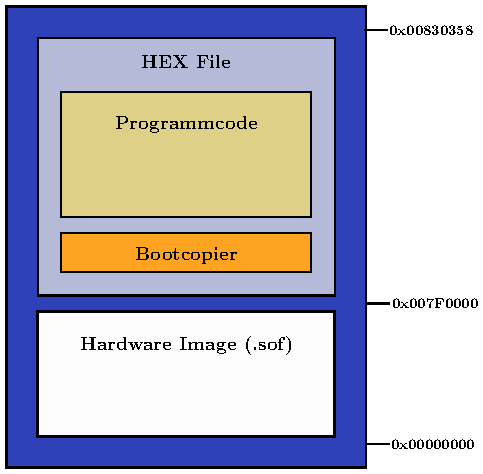
\includegraphics[width=0.45\textwidth]{FlashLayout.pdf}
	\caption{Layout des Flash Speichers} 
	\label{img:FlashLayout}
\end{figure}  

\paragraph{LCD Controller \& Reset}\mbox{}\\

Für das beschreiben des LCD ist die von Terasic bereitgestellte VHDL Komponente\\ LT24\_Controller zuständig. Der Nios II Prozessor steuert diese über das Memory Mapped Interface. Das verwendete Display LT24 von Terasic enthält für das Schreiben des LCD den LCD Treiber ILI9341 von ILITEK. Dieser Chip wird durch den LT24\_Controller über das parallele \SI{16}{Bit} Interface gesteuert. Weiter kann der LCD Chip über den PIO Core LCD Reset zurückgesetzt werden. Wie diese beiden Komponenten in Software angesteuert werden ist in Kapitel \ref{subsec:drivers} genauer beschrieben \cite{LCD_Chip}.

\newpage

\paragraph{Touchscreen}\mbox{}\\

Der Touch Screen Digitizer AD7843 von Analog Devices misst den resistiven Touchscreen des LCD aus und übermittelt die digitalisierten Koordinaten über SPI an den Prozessor. Der Nios II kommuniziert dabei über drei verschiedene IP Cores mit diesem Chip: Der SPI Core \textit{Touch SPI} für die Datenübertragung, der PIO Core \textit{Touch Busy} um den Beschäftigungsstatus des Chips abzufragen und den zweiten PIO Core \textit{Touch Interrupt}, welcher den Nios II über eine Betätigung des Touchscreens informiert. Bei einer Berührung des Touchscreens löst \textit{Touch Interrupt} beim Nios II Prozessor einen Interrupt aus, welcher sofort die Koordinaten über SPI anfordert \cite{Touch_ADC}.
	\subsection{Tonhöhenverarbeitung}\label{subsec:Pitch_Generation}

Die Hauptaufgabe der Komponente \textit{Tonhöhenverarbeitung} ist es das Audiosignal aus dem Rechtecksignal des Tonhöhenoszillators zu generieren. Die \textit{Tonhöhenverarbeitung} nimmt zudem eine Frequenzmessung des Audiosignals vor um diverse Funktionalitäten zu gewährleisten. In Abbildung \ref{img:Blockschaltbild_pitch} ist der Grobe Aufbau der Komponente aufgezeigt. Die genaue Erklärung zu den einzelnen Komponenten ist in den folgenden Abschnitten zu finden.


\begin{figure}[h!]
	\centering
	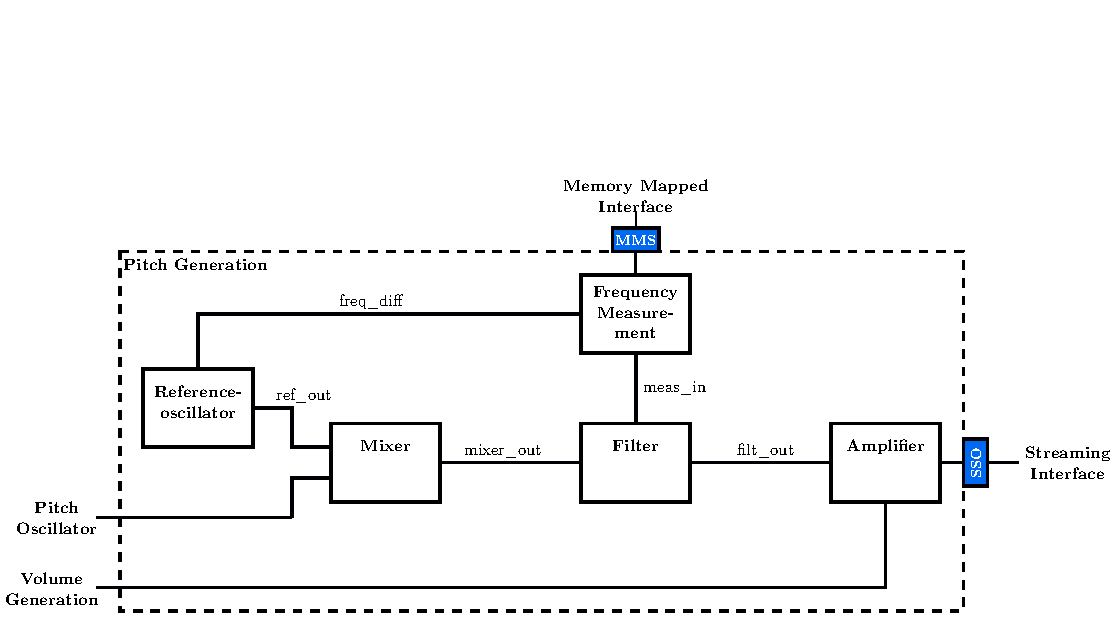
\includegraphics[width=\textwidth]{Blockschaltbild_pitch.pdf}
	\caption{Blockschaltbild der Custom IP \textit{Tonhöhenverarbeitung}} 
	\label{img:Blockschaltbild_pitch}
\end{figure}  



\paragraph{Referenzoszillator}\mbox{}\\

Der \textit{Referenzoszillator} ist wie in der analogen Version aus Kapitel \ref{subsec:Theremin_analog} dafür zuständig ein Sinussignal mit einer Frequenz nahe der des Tonhöhenoszillators zu generieren und an \textit{ref\_out} auszugeben. Er generiert diesen wie schon erwähnt mithilfe des Cordic Algorithmus. Er ist aufgeteilt in zwei Komponenten: der \textit{Cordic Prozessor} und der \textit{Cordic Controller}. Wie diese beiden Komponenten miteinander verbunden sind ist in Abbildung \ref{img:Referenceoscillator} ersichtlich. Beide Komponenten stammen aus dem Projekt 5. Änderungen, welche im Projekt 6 stattfanden, sind entsprechend gekennzeichnet. \\

\begin{figure}[t]
	\centering
	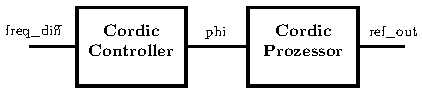
\includegraphics[width=0.53\textwidth]{Referenceoscillator.pdf}
	\caption{Aufbau des Referenzoszillators} 
	\label{img:Referenceoscillator}
\end{figure}  

Der \textit{Cordic Prozessor} ist die eigentliche Implementierung des Cordic Algorithmus wie er in Kapitel \ref{subsec:Cordic} beschrieben wurde. Er muss jedoch für den Einsatz im FPGA leicht angepasst werden. \\
Die Berechnung der Werte für \(\arctan{2^{-i}}\) fand vorgängig statt und ist in eine Lookup Table gespeichert. Dies spart Ressourcen für diese komplizierte Berechnung ein. Wir haben uns entschieden den Algorithmus in einer Pipeline zu implementieren. Dies führt einerseits zu einer höheren maximalen Clockfrequenz, andererseits aber auch zu einer grösseren Signallatenz. Dies ist jedoch nicht problematisch für die gewählte Anwendung, da die Latenz im Nanosekundenbereich ist und später nicht hörbar auffällt. Zuletzt ist eine Multiplikation mit \(2^{-i}\) ganz einfach durch eine Verschiebung um \(i\) Bits nach rechts ersetzbar. Dies spart wiederum Ressourcen ein.\\
Das berechnete Resultat ist als signed Zahl definiert um die Berechnung von negativen Zahlen zu ermöglichen. Sie sind im fixed-point Format und haben \SI{16}{Bit} Länge. Dabei sind von den \SI{16}{Bit} \SI{1}{Bit} Vorzeichen und \SI{15}{Bit} Nachkommastellen. Dies entspricht einem Zahlenbereich von -1 bis 0.999969. Die berechneten Werte gibt der \textit{Cordic Prozessor} an \textit{ref\_out} aus.

Für die Berechnung der Sinuswerte muss ein Winkelwert berechnet werden, der mit der Zeit so ändert, dass sich am Ausgang des Cordic Prozessor ein Sinus mit der gewünschten Frequenz ergibt. Der berechnete Winkelwert wird an \textit{phi} ausgegeben. Für diese Aufgabe ist der \textit{Cordic Controller} zuständig. Bei mit der Zeit linear ansteigendem Winkelwert ergibt sich am Ausgang die gewünschte Sinusform. Wichtig ist jedoch, dass der Cordic Algorithmus nur für Winkelwerte zwischen \(-\pi/2\) und \(\pi/2\) oder anders für Werte im ersten und zweiten Quadranten konvergiert. Die Lösung für dieses Problem ist in Abbildung \ref{img:Cordic_phi} ersichtlich. 
Als erstes wird der Sägezahn Winkel berechnet. Für den linearen Anstieg des Winkels zählt der \textit{Cordic Controller} einen Zähler mit einer bestimmten Schrittweite jeden Clockzyklus hoch. Der wrap-around des Zählers ist dabei erwünscht um den Sprung zwischen dem II und III Quadranten zu erzielen. Der Schrittwert ergibt sich wie folgt:

\begin{equation}
step = \frac{2^{n+1}f_{sig}}{f_{clk}}
\label{equ:cordic_step}
\end{equation} 

Wobei \(n\) die Anzahl Bits des Wertebereichs des Dreiecks Winkels ist, \(f_{sig}\) die gewünschte Frequenz des generierten Signals und \(f_{clk}\) die Clock Frequenz des FPGA.

Nun kommt die bereits erwähnte Einschränkung des Cordic Algorithmus ins Spiel. Die berechneten Werte des Sägezahnwinkels zwischen dem II und III Quadranten konvergieren nicht. Aus diesem Grund konvertiert der \textit{Cordic Controller} diesen Winkel in den Dreieckswinkel. Sind die beiden vordersten Bits entweder \(01\) oder \(10\) befindet sich der Winkelwert im II respektive III Quadranten. Um in diesem Fall den Dreieckswinkel zu erhalten invertiert der \textit{Cordic Controller} alle Bits ausser dem most-significant Bit. Wie man sich leicht davon überzeugen kann ergibt der Dreieckswinkel denselben Sinusverlauf wie der Sägezahnwinkel bei einer Sinusrechnung ohne die erwähnten Einschränkungen. \cite{Cordic}

Um die Kalibrierung und den Glissandoeffekt für das Theremin zu ermöglichen waren im Projekt 6 kleine Anpassungen am \textit{Cordic Controller} nötig. Wie zuvor hat der Controller eine fixe Frequenz implementiert, welche in der Grössenordnung \SI{550}{kHz} liegt. Jedoch legt die Frequenzmessungskomponente nun eine Differenz über einen Eingang an den Cordic Controller an um die zuvor genannten Features über den Referenzoszillator zu ermöglichen.


\begin{figure}[t]
	\centering
	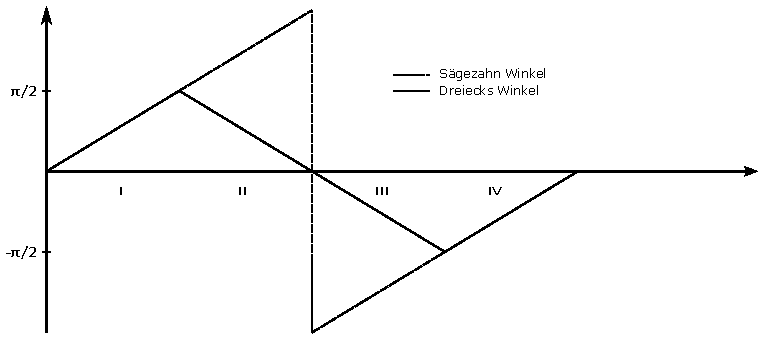
\includegraphics[width=0.8\textwidth]{Cordic_phi.pdf}
	\caption{berechneter Winkel \textit{phi} des Cordic Controllers in Funktion der Zeit} 
	\label{img:Cordic_phi}
\end{figure}  


\paragraph{Mischer}\mbox{}\\

Die Implementation des \textit{Mischers} ist dank der Entscheidung für die Rechteckform des Tonhöhenoszillatorsignals sehr einfach. Über einen GPIO liest der Mischer das Signal des Tonhöhenoszillators ein und verrechnet es mit dem generierten Sinus \textit{ref\_out}. Eine \textit{1} des Rechtecks wird dabei als die Zahl \textit{1} und eine \textit{0} als die Zahl \textit{-1} interpretiert. Die Multiplikation zwischen der \textit{1} und \textit{ref\_out} ist dabei nicht nötig und eine Multiplikation mit \textit{-1} erzielt der Mischer durch das Bilden des Zweierkomplement von \textit{ref\_out}.

\paragraph{Filter}\mbox{}\\

Im Projekt 5 war das \textit{Filter} ein einzelnes CIC-Filter mit dem Dezimationsfaktor 1000. Dies hatte zur Folge, dass viel Aliasing entstand. Um dieses zu verringern haben wir uns im Projekt 6 für den Aufbau aus Abbildung \ref{img:Filter_Pitch} entschieden. Die drei Filter CIC 1 bis CIC 3 sind Instanzen einer CIC-Filter Komponente. Diese Komponente stammt weitestgehend aus dem Projekt 5, ist jedoch auf mehr Modularität erweitert. Die Parameter der drei Instanzen sind in Tabelle \ref{tab:cic_pitch} ersichtlich. Da es bei CIC-Filtern wie in Kapitel \ref{subsec:CIC_Filter} beschrieben, um deren Nullstellen zu Aliasing kommt, sind diese Filter so eingestellt, dass sich die Oberwellen des Rechteck möglichst nicht in deren Nähe befinden. Bei \textit{CIC 1} wurde eine höhere Ordnung gewählt um am Anfang eine stärkere Dämpfung zu erzielen. Die Anzahl Ausgangsbits erhält man mit Formel \ref{equ:cic_bitgrowth} in Kapitel \ref{subsec:CIC_Filter}.\\
Zuletzt haben wir noch ein FIR-Filter implementiert um das Signal auf 48kHz unter abzutasten. Das Filter hat eine Passfrequenz von \SI{2}{kHz} und eine Stopfrequenz von \SI{24}{kHz} mit einer Dämpfung von 55dB. Wir entschieden uns die Koeffizienten mit dem \textit{filterDesigner Tool} von Matlab zu berechnen und als \SI{27}{Bit} signed Zahlen in einer Lookup Table zu speichern. Wir wählten deshalb \SI{27}{Bit}, da im FPGA eine solche Multiplikation noch knapp in einen DSP Block integriert werden kann. \cite{Cyclone_V}
Weswegen der Ausgang Frequenzmessung nach dem zweiten CIC-Filter gewählt wurde ist in einem späteren Abschnitt beschrieben.


\begin{figure}[t]
	\centering
	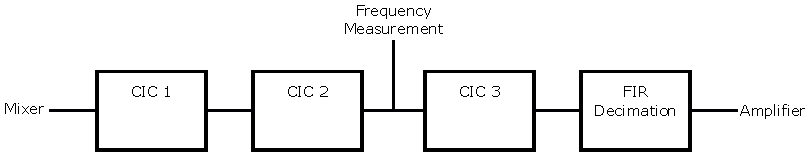
\includegraphics[width=1\textwidth]{Filter_pitch.pdf}
	\caption{Aufbau des Filters in der Komponente Pitch Generation} 
	\label{img:Filter_Pitch}
\end{figure}  

\begin{table}[t]
	\centering
	\caption{Parameter der drei CIC-Filter}
	\label{tab:cic_pitch}
	\begin{tabular}{l|l|l|l|l}
		\textbf{Komponente} & \textbf{Dezim.Fakt.} & \textbf{Ordnung} &  \textbf{Ausgangsfreq.} & \textbf{Ausgangsbits}\\
		\hline\hline
		CIC 1 & 5 & 2 & \SI{10.8}{MHz} & \SI{21}{Bits}  \\ \hline
		CIC 2 & 9 & 1  & \SI{12}{MHz} & \SI{25}{Bits}  \\ \hline
		CIC 3 & 5 & 1 & \SI{240}{kHz} & \SI{28}{Bits}  \\ \hline	
	\end{tabular}
\end{table}

\paragraph{Verstärker}\mbox{}\\

Die Komponente \textit{Verstärker} ist dafür zuständig beim Signal \textit{filt\_out} den Gain der CIC-Filter zu kompensieren und anschliessend dieses mit der Dämpfung, welche die Lautstärkeverarbeitung liefert, zu multiplizieren. In Abbildung \ref{img:Zero_Cross} ist eine Problematik aufgezeigt, welche auftritt, wenn man die Dämpfung zu beliebigen Zeiten wechselt. Links ist zu sehe, was passiert, wenn die Dämpfung beim höchsten Wert der positiven Halbwelle ändert. Diese Sprünge im Signal treten dann als hörbares Knacksen auf. Um dies zu verhindern ist eine Erkennung von Nulldurchgängen implementiert, dass wie in der Abbildung rechts die Dämpfungen nur bei diesen Nullstellen ändern. Da der Codec ein offsetbehaftetes Signal verlangt muss das most-significant Bit des Signal getoggelt werden um dies zu bewerkstelligen. Diese Komponente enthält zudem die Kommunikation mit dem Streaming Interface. \\
Die Dämpfung des Audiosignals könnte auch über den Codec gemacht werden. Weshalb dies nicht möglich ist, ist in Kapitel \ref{subsec:audio} beschrieben. 
	
\begin{figure}[h!]
	\centering
	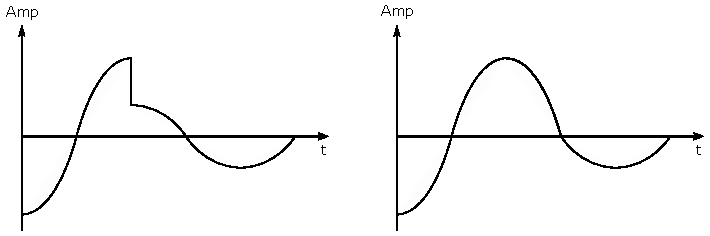
\includegraphics[width=1\textwidth]{Zero_Cross.pdf}
	\caption{Unterschied Dämpfungswechsel (links ohne und rechts mit Nullstellenerkennung)} 
	\label{img:Zero_Cross}
\end{figure}  

\newpage

\paragraph{Frequenzmessung, Kalibration \& Glissandoeffekt}\mbox{}\\

Die Komponente \textit{Frequenzmessung} hat mehrere Aufgaben und ist diejenige Komponente mit welcher über den Nios II Prozessor die gesamte \textit{Tonhöhenverabreitung} gesteuert werden kann. Der Aufbau dieser Komponente ist in Abbildung \ref{img:freq_meas_pitch} aufgezeigt.\\
Zum einen wird hier die Frequenzmessung durchgeführt. Dies geschieht über die drei Komponenten FIR, Periodenzähler und Goldschmidtdividierer. FIR ist wie der Name sagt ein FIR Filter. Dieses ist nötig um das Signal aus den CIC-Filtern, welches noch hochfrequente Anteile enthält zu filtern. Das FIR Filter hat eine Passfrequenz von \SI{2}{kHz} eine Stopfrequenz von \SI{40}{kHz} und eine Dämpfung von 30dB. Das Filter ist mit dem \textit{filterDesigner} Tool in Matlab berechnet. Wir haben entschieden die Filterkoeffizienten als fixed-point signed Zahlen in einem Array mit \SI{18}{bit} länge abzuspeichern. Auf dieser Koeffizientenlänge kann Quartus die DSP-Blöcke so nutzen, dass nach der Multiplikation des Signals mit den Koeffizienten die Resultate gleich in den Blöcken addiert wird. Dies ermöglicht längere Multiplikationsketten. \cite{Cyclone_V}\\
Anschliessend wird das Signal \textit{fir\_out} im \textit{Periodenzähler} ausgemessen. Dieser zählt von Nulldurchgang zu Nulldurchgang einen Zähler hoch. Bei einem Nulldurchgang wird der Wert dieses Zählers am Signal \textit{per\_cnt} ausgegeben. Der Zählerwert entspricht der Anzahl Abtastwerte des Signals in einer Signalperiode. \\
Das Signal hat eine Abtastfrequenz von \SI{1.2}{MHz}. Dividiert man diese Abtastfrequenz durch die zuvor gezählte Anzahl Abtastperioden erhält man die Frequenz des Signals.\\ Um diese Division zu berechnen haben wir uns entschieden den Goldschmidt Algorithmus aus Kapitel \ref{subsec:Goldschmidt} einzusetzen. Dieser hat den Vorteil, dass er auch Nachkommastellen berechnen kann um die nötige Genauigkeit bei den tiefen Frequenzen zu erreichen wie in Kapitel \ref{subsec:Musiktheorie} beschrieben. Dass die Berechnungsdauer des Algorithmus nicht für alle Zahlen gleich ist, ist nicht Problematisch, da diese Zeiten im Nanosekundenbereich liegen und nicht hörbar sind. Der Messbereich der Frequenzmessung fängt bei \SI{100}{Hz} an und geht bis \SI{10}{kHz}. Alle Frequenzen darunter oder darüber zeigen \SI{100}{Hz} respektive \SI{10}{kHz} an.

\begin{figure}[h!]
	\centering
	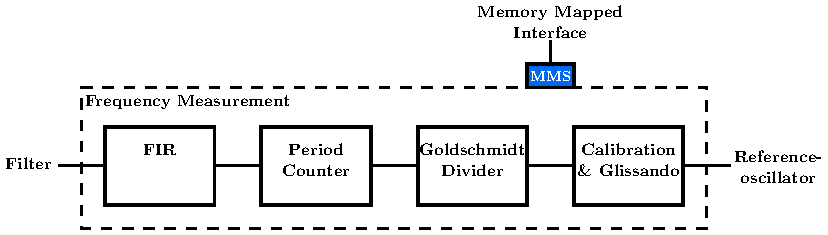
\includegraphics[width=1\textwidth]{freq_meas_pitch.pdf}
	\caption{Aufbau der Frequenzmessung, Kalibration und Glissandoeffekt in der Komponente Pitch Generation} 
	\label{img:freq_meas_pitch}
\end{figure}  

Die gemessene Frequenz wird anschliessend in der Komponente \textit{Kalibration \& Glissando} benötigt. Diese ist dafür zuständig einerseits die Tonhöhe zu kalibrieren und andererseits den Glissando-Effekt zu steuern. Um die Frequenz des Audiosignals für diese Funktionen zu verändern verstimmt die Komponente den Referenzoszillator entsprechenden. Kalibration \& Glissando addiert die Differenz welche den Glissandoeffekt hervorruft und die Änderung welche während der Kalibration berechnet wurde und übergibt das Resultat dem Referenzoszillator. Diese wird von nun an als Frequenzdifferenz bezeichnet. Die Steuerung dieser Funktionen ist als State-Machine aufgebaut wie in Abbildung \ref{img:state_event_Cal_Glis} zu sehen ist. 
Dabei sind die States reset, check, sign und diff für die Kalibration zuständig und freq range, step und step count für den Glissando-Effekt zuständig. Es folgt eine Erklärung, was in den einzelnen Zuständen geschieht:

\textbf{Idle}:
Der Idle State setzt die Frequenzdifferenz auf die berechnete Differenz der Kalibrierung. Der Anteil des Glissando-Effekts wird auf 0Hz gesetzt.

\textbf{reset}:
Der alte Kalibrationswert wird gelöscht und gewartet bis eine neue Frequenzmessung abgeschlossen ist.

\textbf{check}:
Da die Messung Frequenzen unter \SI{100}{Hz} immer als \SI{100}{Hz} angibt, muss die Komponente diese erkennen. Bei einer Messung von \SI{100}{Hz} inkrementiert die Komponente Calibration \& Glissando die Frequenzdifferenz um \SI{400}{Hz}. Dies führt dazu, dass bei der nächsten Messung das Signal nicht mehr in dem Bereich liegt, in dem die Messung immer \SI{100}{Hz} misst.

\textbf{sign}:
Für die in Kapitel \ref{sec:Konzept} beschriebene Spielweise, dass mit kleinerer Distanz zur Antenne die Tonhöhe steigt, ist der State sign zuständig. Ist der Referenzoszillator so eingestellt, dass dessen Frequenz kleiner ist als die des Tonhöhenoszillators, so würde bei Annäherung des Spielers an die Antenne die Frequenz des Audiosignals zuerst sinken, bis die beiden Oszillatorfrequenzen gleich sind. Dies, da die Frequenz des Tonhöhenoszillators mit kleinerem Abstand immer mehr sinkt. Anschliessend würde sie wieder steigen, da der Tonhöhenoszillator kleiner ist als der Referenzoszillator. Um zu erkennen ob dies der Fall ist, subtrahiert die Komponente \SI{100}{Hz} von der Frequenzdifferenz. Ist die nachfolgende Messung grösser geworden, bedeutet dies, dass der Referenzoszillator kleiner war als der Tonhöhenoszillator. Nun kann ganz einfach die gemessene Frequenz verdoppelt und zu der Frequenzdifferenz addiert werden, damit der Referenzoszillator die grössere Frequenz hat.

\textbf{diff}:
Nach den letzten drei States ist nun sichergestellt, dass der Referenzoszillator grösser ist als der Tonhöhenoszillator. Jedoch sollen ja diese beiden Oszillatoren aufeinander abgestimmt sein. Dazu wird abwechslungsweise die Frequenzdifferent um einen kleinen Schritt dekrementiert und danach die Frequenz gemessen. Wir haben uns dafür entschieden, dass wenn die Messung \SI{120}{Hz} unterschreitet die Kalibration abgeschlossen ist. Dies da Töne unterhalb dieser Frequenz sehr merkwürdig klingen.

\textbf{freq range}:
Der State freq range ist dafür zuständig herauszufinden, welcher diskrete Ton der gewählten Tonleiter (normal oder pentatonisch) am nächsten zur gemessenen Frequenz ist. Die Frequenz wird dabei mit einer Lookup-Table mit allen Grenzen zwischen den Tönen verglichen. ist die Frequenz ausserhalb des gewählten Frequenzbereich wird hier abgebrochen und in den State idle gewechselt.

\textbf{step}:
Der State step bestimmt die Schrittgrösse, welcher im nächsten State für die Annäherung nötig ist. Die Schrittgrössen für alle Töne sind im Vorhinein berechnet als \SI{1}{Cent} Differenz zum eigentlichen Ton. Würde überall die gleiche Schrittgrösse genommen, wäre das Aufschliessen bei hohen Tönen extrem langsam und bei tiefen Tönen so schnell, dass kein Übergang hörbar ist. 

\textbf{step count}:
Der letzte State verrechnet die Frequenzdifferenz in vorgegebenen Intervallen mit dem zuvor bestimmten Step, bis auf den Ton aufgeschlossen ist. Hat die Frequenzmessung jedoch während dem Zählen eine neue Frequenz gemessen wird in den State freq range gewechselt. Erreicht das Aufschliessen bevor eine neue Messung stattfand einen Unterschied von unter \SI{6}{Cent} zu der anzunähernden Frequenz, stoppt das Zählen bis zu einer neuen Messung.

\begin{figure}[h!]
	\centering
	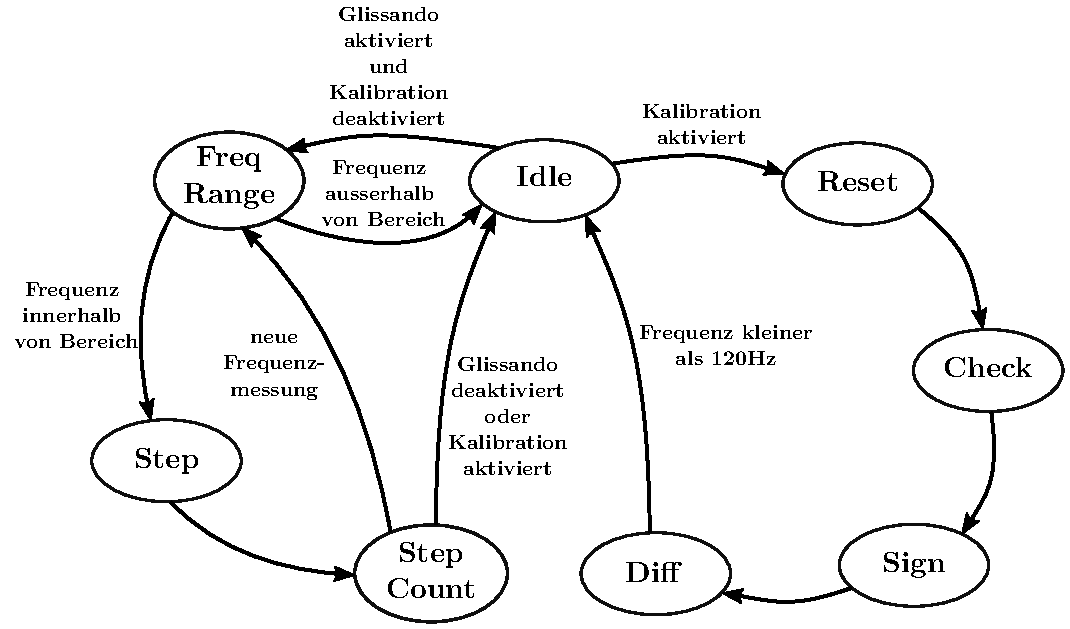
\includegraphics[width=1\textwidth]{state_machine_Cal_Glis.pdf}
	\caption{State Event Diagramm der Kalibration \& Glissando Komponente} 
	\label{img:state_event_Cal_Glis}
\end{figure} 

\paragraph{Register}\mbox{}\\
Um mit der Komponente \textit{Tonhöhenverarbeitung} über das Memory-Mapped Interface kommunizieren zu können haben wir folgende Register definiert:

\begin{table}[H]
	\centering
	\caption{Zusammenfassung der Register}
	\label{tab:Registers_pitch}
	\begin{tabular}{l|l|l|l|l|l|l}
		\textbf{Register} & \textbf{Adresse} & \textbf{R/W} &	\multicolumn{4}{l}{\textbf{Bits}} \\\cline{4-7}
						  &					 &				& \textbf{31-3}  & \textbf{2} & \textbf{1} & \textbf{0}\\ 
		\hline \hline
		
		cntrl\_reg & 00 & R/W & X & scale & cal & glis \\ 
		\hline
		freq\_data\_reg & 01 & R & \multicolumn{4}{l}{Frequenz} \\
		\hline
		delay\_data\_reg & 10 & W & \multicolumn{4}{l}{Verzögerung} \\
	\end{tabular}
\end{table}

\begin{table}[H]
	\centering
	\caption{Control Register Flags}
	\label{tab:Register_pitch_cntrl}
	\begin{tabular}{l|l|l|l}
		\textbf{Bits} & \textbf{Kürzel} & \textbf{R/W} &	\textbf{Beschreibung}\\
		\hline \hline
		
		0 & glis & W &  1 = Glissando-Effekt aktiviert \\ 
		  &      &   &  0 = Glissando-Effekt deaktiviert \\ 
		\hline
		1 & cal & R/W &  1 = Kalibration aktiviert \\ 
		  &     &     &  0 = Kalibration beendet \\ 
		\hline
		2 & scale & W &  1 = Pentatonische Tonleiter \\ 
		 &     &       &  0 = Normale Tonleiter \\ 
		\hline

	\end{tabular}
\end{table}

Das Register \textit{freq\_data\_reg} enthält die Frequenz für die Anzeige der Spielgenauigkeit. Mehr dazu in Kapitel \ref{subsec:audio}. \\
Das Register \textit{delay\_data\_reg} enthält die Einstellung für die Zeit, die der Glissando-Effekt benötigt um die Töne zu korrigieren. Es können Werte von 0 bis 9 geschrieben werden um diese Zeit zu verändern.


	\subsection{Volume Generation}\label{subsec:Volume_Generation}
bla bla




\pagebreak

\clearpage
\section{Validierung}\label{sec:Validierung}
In diesem Kapitel wird zuerst das Antennenoszillator PCB getestet. Anschliessend wird mit Simulationen des VHDL Codes, durch berechnen der jeweiligen Spektren der Zwischenresultate, deren gesamte Funktion getestet. Zum Schluss wird auf die Inbetriebnahme und das Debugging Bezug genommen.
	\subsection{PCB}\label{subsec:PCB}
bla bla


	\subsection{Frequenzmessung}\label{subsec:Frequenzmessung}
bla bla

	\subsection{Glissando Effekt}\label{subsec:Glissando_Effekt}
bla bla


	\subsection{Ton Display}\label{subsec:Ton_Display}
bla bla



\pagebreak


\clearpage
\section{Schlusswort}\label{sec:Schlusswort}
Im Rahmen des Projekt 5  wurde eine digitale Plattform für die Verarbeitung von Signalen einer Thereminantenne entwickelt. Alle Komponenten ausser der Antennenoszillator wurden in VHDL realisiert. Die VHDL Komponenten wurden so realisiert, dass diese im Projekt 6 weiter gebraucht werden können.
Momentan lässt sich das Theremin ohne Lautstärkeantenne spielen. Über zwei Taster kann der digitale Referenzoszillator manuell auf die Frequenz des Tonhöhenoszillator abgestimmt werden. Sobald das Theremin kalibriert ist kann es Töne von ca. 100-2000Hz spielen. 
Die Ziele welche in der Projektklärung definiert wurden konnten erfüllt werden. Bei der kontinuierlichen Tongenerierung gibt es noch eine Unschönheit bei der Ansteuerung des Codec. Es ist im generierten Ton ein Knacken zu hören, welches auf einen Fehler in der Ansteuerung des verwendeten Codec zurückzuführen ist. Dieser Fehler besteht nach wie vor. Jedoch wird diese Ansteuerung in Projekt 6 sowieso anders realisiert.

Im Projekt 6 wird die zweite Antenne implementiert, um gleichzeitig die Lautstärke einstellen zu können. Des weiteren soll es möglich sein diskrete Töne zu spielen. Dieser Modus soll es Anfängern ermöglichen bekannte Melodien nachspielen zu können. \\
Damit das theoretische Wissen aus dem Fach digitale Schaltungstechnik (dst) in die Praxis umgesetzt werden kann, wird ein Nios Soft Core Prozessor implementiert. Dieser übernimmt die Ansteuerung des Codec und die Modus Verwaltung. Beim starten des Theremin soll ein automatisches Tuning des Referenzoszillators stattfinden. Dazu wird der digitale Referenzoszillator auf die Frequenz des Antennenoszillator abgestimmt. Um das Theremin für Messen zu verwenden wird das DE1-SoC Board und die Antennenoszillatoren mit den Antennen in ein ansprechendes Gehäuse verbaut. Die Antennen sollen abgeschraubt werden können um einen komfortablen Transport zu ermöglichen.

Als erstes wird im Projekt 6 mit der Implementierung der Lautstärkeantenne auf dem FPGA und dem Redesign des PCB begonnen. Zudem muss Recherche in das Thema Nios Soft Core Prozessor angestellt werden, um diesen später implementieren zu können. 







\pagebreak

\section{Ehrlichkeitserklärung}\label{sec:Ehrlichkeitserklärung}
Mit der Unterschrift bestätigen die Unterzeichnenden Teammitglieder, dass die vorliegende Projektdokumentation selbstständig im Team und ohne Verwendung anderer, als der angegebenen Hilfsmittel verfasst wurde, sämtliche verwendeten Quellen erwähnt und die gängigen Zitierregeln eingehalten wurden. Eine Überprüfung der Arbeit auf Plagiate mithilfe elektronischer Hilfsmittel darf vorgenommen werden.


\vspace{20mm}


\begin{center}
		\renewcommand{\arraystretch}{1}
	\begin{tabular}{lp{5em}l} 
  
		
		Unterschrift:   && Ort, Datum: \\
		&&\\
		\hspace{5cm}   && \hspace{5cm} \\\cline{1-1}\cline{3-3}
		&&\\
		&&\\
		Unterschrift:   && Ort, Datum: \\
		&&\\
		\hspace{5cm}   && \hspace{5cm} \\\cline{1-1}\cline{3-3}
		&&\\
		&&\\

  
  \ \\
 \end{tabular}
 \end{center}





\pagebreak


\clearpage
%%---BIBLIOGRAPHY------------------------------------------------------------------------
{\sloppypar
\printbibliography[heading=bibintoc]
\label{sec:lit}
%\selectlanguage{ngerman}				%ngerman or english
%\printbibliography
}

%%---APPENDIX----------------------------------------------------------------------------
\begin{appendix} 


\end{appendix}


%%---NOTES for DEBUG---------------------------------------------------------------------
\ifdraft{%Do this only if mode=draft
%%requires \usepackage{todonotes})
\newpage
\listoftodos[\section{Todo-Notes}]
\clearpage
}
{%Do this only if mode=final
}

\end{document}
